\section{Hashes}
As we have seen in the previous chapters, if we want to guarantee both confidentiality and authentication with public crypto, the sender needs to encrypt the message with his private key (authenticity) and with the receiver public key (confidentiality). To reduce the computational burden we can use hash functions.\\
A hash function is a function that maps an arbitrary length input into a finite length output of $2^n$ bits (called \textit{message digest} or \textit{hash}).
If Alice wants to send a message to Bob, we can exploit hash functions in the following way:
\begin{wrapfigure}{r}{0.3\textwidth}
\vspace{50pt}
\fbox{
\includegraphics[scale=0.40]{images/hash.png}}
\end{wrapfigure}
\begin{enumerate}
    \item Alice computes the hash $h$ of the message $m$, encrypts it with her private key, and creates the new message $m'=m||E(D_A,h)$
    \item Alice encrypts $m'$ with the public key of Bob, generating $c=E(E_B,m')$
    \item Bob receives $c$, decrypts it with his private key, obtaining $m'$
    \item Bob separates $m$ from $E(D_A,h)$ and decrypts the latter with Alice's public key, obtaining $h$
    \item Bob verify the authenticity of the message simply computing the hash of the message $m$ and comparing it with $h$
\end{enumerate}
%\begin{center}
%    \includegraphics[scale=0.7]{hash.png}
%\end{center}

\subsection{Hash functions requirements}
A good hash function has by definition the following property:
\begin{itemize}
    \item \textbf{One-Wayness}: For any given image $h$ it is computationally infeasible to find pre-image $x$ s.t. $H(x) = h$
    \item \textbf{Weak collision resistance}: For any given pre-image $x$ it is computationally infeasible to find a pre-image $y\neq x$ with $H(x)=H(y)$
    \item \textbf{Strong collision resistance}: it is computationally infeasible to find any pair of pre-images $(x,y)$ s.t. $H(x)=H(y)$
\end{itemize}
\subsection{Birthday Attack}
It is clear that we need weak collision resistance property to obtain authenticity, but why do we need the strong collision resistance? The reason is that, without this property, it is possible to perform a birthday attack. A birthday attack is a type of cryptographic attack that exploits the mathematics behind the \textit{birthday problem}.
\subsubsection{Birthday Problem}
The birthday problem asks for the probability that, in a set of $n$ randomly chosen people, at least two will share a birthday. The birthday paradox is that, counterintuitively, the probability of a shared birthday exceeds 50\% in a group of only $23$ people. This can be proved using statistics:
\begin{itemize}
    \item Given $n$ people and $k$ days in a year, we have a probability\\ $P=1-\frac{(k-1)!}{k^{n-1}(k-n)!}$ that two of them share the birthday
    \item with $n=23$ and $k=365$, $P=1-\frac{364!}{365^{22}(365-23)!}\approx1-0.49=0.51$
\end{itemize}
\subsubsection{Applications}
We can exploit the birthday problem in the following way:
\begin{itemize}
    \item Prepare $2^{m/2}$ variations of valid and fraudulent messages each
    \item This should give us a $50\%$ chance of finding collision between a valid and a fraudulent message
    \item Now we can get someone to sign hash the valid message and then replace it with the fraudulent one
\end{itemize}

\newpage
\subsection{Hash Algorithms}
A generic hash algorithm works in the following way:
\begin{center}
    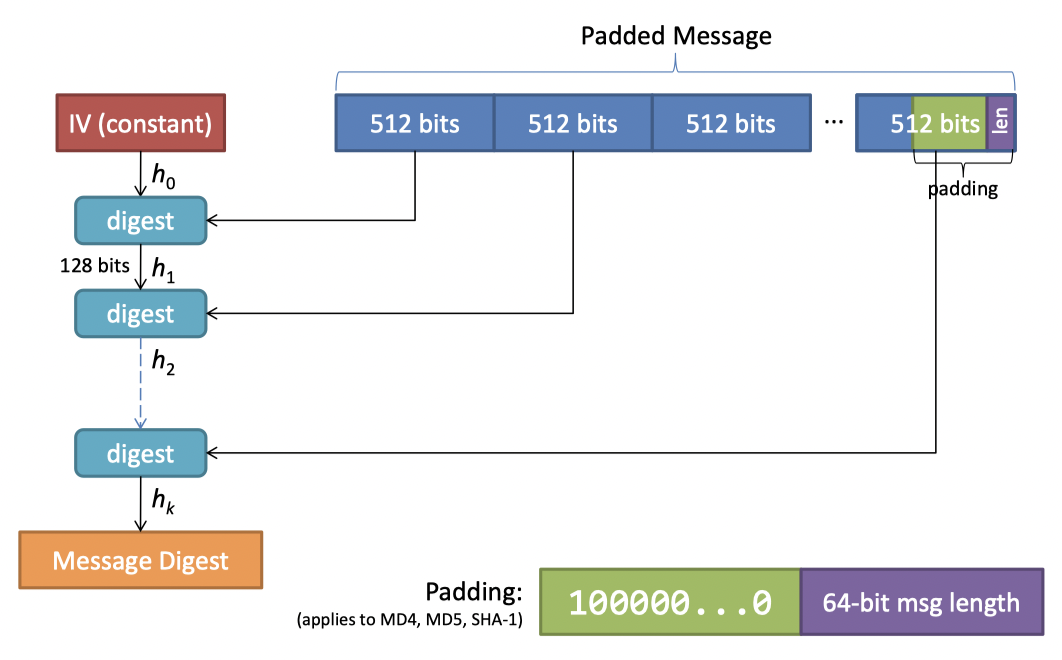
\includegraphics[scale=0.6]{hashfunc.png}
\end{center}

\subsubsection{MD5}
\begin{center}
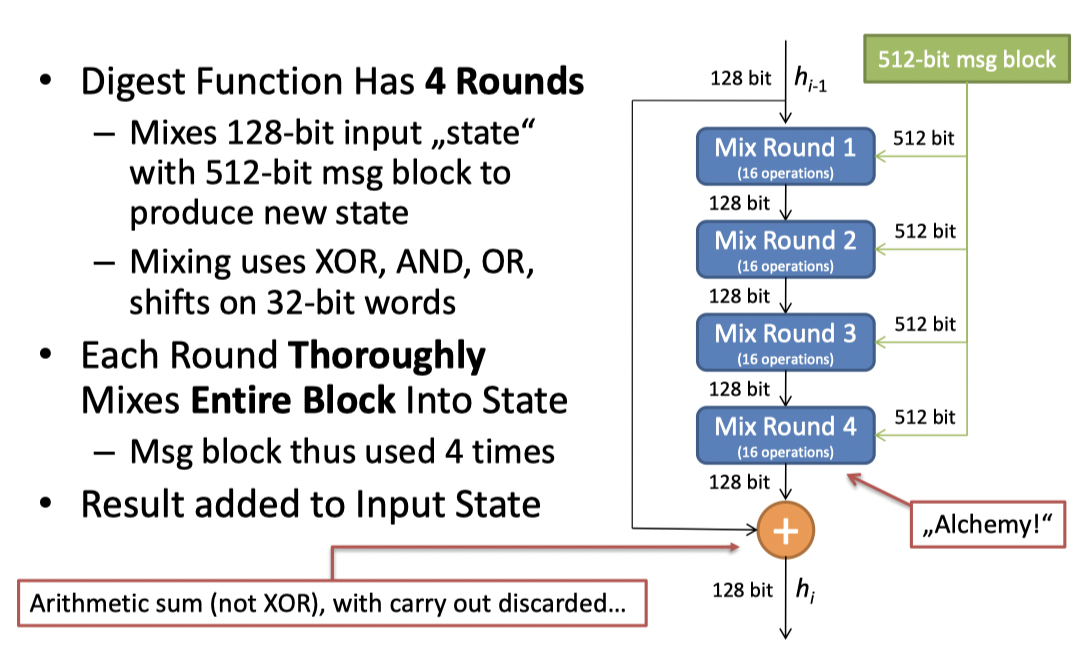
\includegraphics[scale=0.7]{md5.png}
    
\end{center}
\subsubsection{SHA1}
\begin{center}
    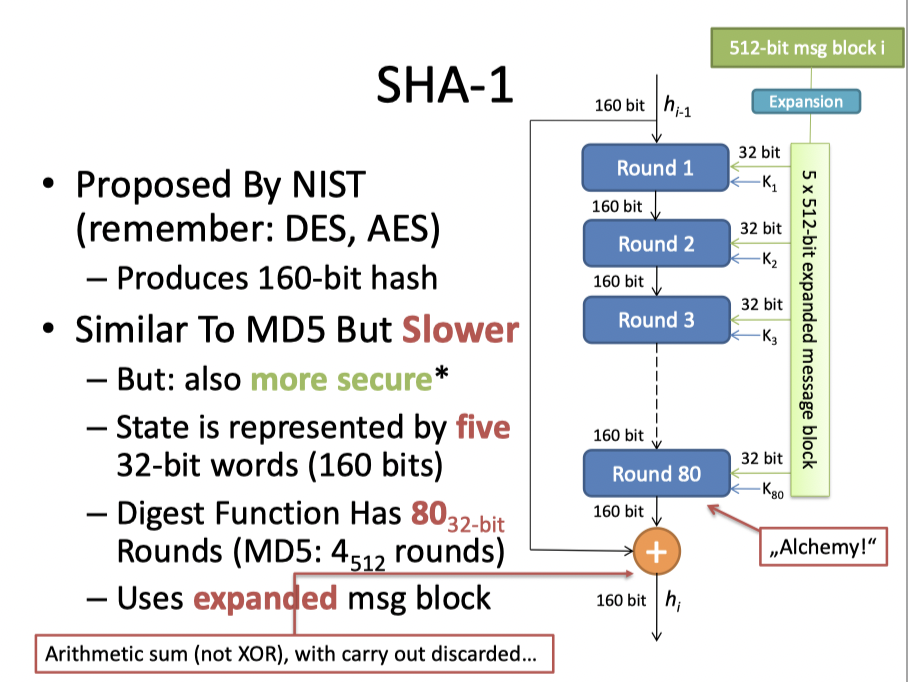
\includegraphics[scale=0.5]{sha1.png}    
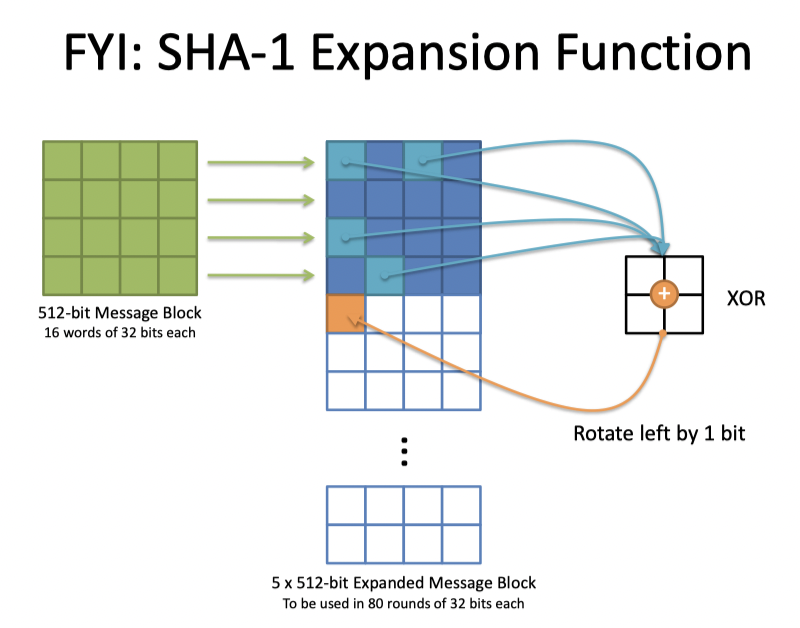
\includegraphics[scale=0.3]{sha1expfunc.png}
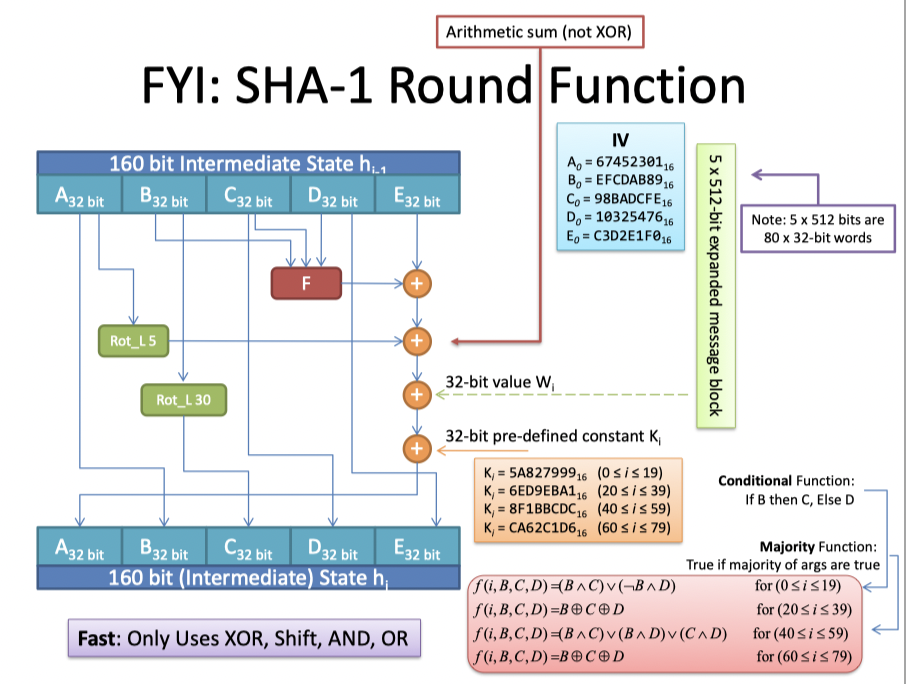
\includegraphics[scale=0.5]{sha1round.png}
\end{center}


